\chapter{Vassiliev invariants and chord diagrams}
\label{ch:vassiliev-invariants-and-chord-diagrams}

\lettrine{\libertineInitialGlyph{V}}{assiliev} invariants are sophisticated to define in terms of the space of knots from the introduction, but the axiomatic definition of Birman-Lin \cite{knot-polynomials-and-vassilievs-invariants} is much simpler. The definition also illustrates an analogy first made by Bar-Natan \cite{on-the-vassiliev-knot-invariants} in which Vassiliev invariants are ``polynomial invariants''. This is not meant in the sense that Vassiliev invariants take values in a polynomial ring (like say, the Jones polynomial), but rather that Vassiliev invariants have special properties not shared by all invariants, just as polynomial functions have special properties not shared by all functions.

\section{Singular Knots}
\label{sec:singular-knots}

\begin{definition}
	A \textbf{singular knot} is an immersion of \(S^{1}\) into \(\R^{3}\) which fails to be an embedding at finitely many singularities, and where the singularities are double-points and transverse. When a singular knot has \(m\) such singularities, we call it \textbf{\(m\)-singular}.
\end{definition}

\begin{remark}
	\label{rem:other-singularities}
	Immersions with other types of singularities, are excluded from this definition, so the word ``singular'' in ``singular knot'' refers specifically to double point singularities. In particular immersions with
	\begin{enumerate}
		\item triple points
		\item points with vanishing derivative
	\end{enumerate}
	are excluded from the definition.
\end{remark}

A singular knot with one double point is very close to two other knots, one where it's replaced by a positive crossing and one by a negative. If the conditions are right, we can extend a knot invariant to an invariant of singular knots by ``taking its derivative''.

\begin{definition}
	\label{def:derivative}
	The \textbf{derivative} \(\delta\) of a differentiable \(m\)-singular knot invariant \(f\) is
	\[\delta f \left( \double \right) = f \left( \poscross \right) - f\left( \negcross \right).\]
\end{definition}

What are the conditions? For this to be a well-defined operation, it mustn't matter which double point we choose.

\begin{definition}
	\label{def:differentiable-invariant}
	An invariant \(f\) of \(m\)-singular knots is \textbf{differentiable} if
	\begin{equation}
		\label{eq:diff}
		\tag{\biolinum{DIFF}}
		f \left( \poscross \ \double \right) - f\left( \negcross \ \double \right) = f \left( \double \ \poscross \right) - f\left( \double \ \negcross \right).
	\end{equation}
\end{definition}

If an invariant of \(m\)-singular knots is differentiable, so is its derivative, so it can be extended to any number of double points.

Rather than thinking about functions on knots satisfying certain relations, the modern version of this subject takes the philosophy of imposing relations on the objects directly.

\begin{definition}
	\label{def:differentiable-knot}
	Define \(\mathcal{K}_{m} = \operatorname{span}(\{m\text{-singular knots}\})\) modulo the following boundary relation (also known as a codifferentiability relation):
	\begin{equation}
		\label{eq:boundary}
		\tag{\biolinum{DIFF*}}
		\poscross \ \double - \negcross \ \double = \double \ \poscross - \double \ \negcross.
	\end{equation}

	From now on, we will refer to elements \(\mathcal{K}_{m}\) as \(m\)\textbf{-singular knots}, i.e. the \ref{eq:boundary} relation will be implicit in everything.
\end{definition}

\begin{definition}
	\label{def:boundary}
	The \textbf{boundary} operation is the map \(\partial : \mathcal{K}_{m} \to \mathcal{K}_{m - 1}\) defined by
	\[ \double \longmapsto \poscross - \negcross .\]
\end{definition}

\begin{remark}
	The derivative operation and the \ref{eq:diff} relation are dual to the boundary operation and the \ref{eq:boundary} relation. For example, a differentiable invariant of knots is the same as a invariant of knots in \(\mathcal{K}_{m}\).
\end{remark}

Any knot invariant, \(f\) can be extended to an invariant \(f^{(m)}\) of \(m\)-singular knots by the Vassiliev skein relation
\[f^{(0)} = f\]
and
\[f^{(m + 1)}\left(\double\right) = f^{(m)}\left(\poscross\right) - f^{(m)}\left(\negcross\right).\]
Often, we omit the superscript and write
\[f\left(\double\right) = f\left(\poscross\right) - f\left(\negcross\right).\]

The Vassiliev skein relation extends a knot via its derivative, or chooses a value on \((m + 1)\)-singular knots to agree with the difference of values on its boundary.

% TODO: Could move later, even.
\begin{definitions}
	\begin{enumerate}
		\item A knot invariant \(V\) is a \textbf{Vassiliev invariant} of order (or type) \(m\) if when extended to singular knots via the Vassiliev skein relation, there is an integer \(m\) such that
		\[V\biggl( \underbrace{\double \cdots \double}_{{\scriptscriptstyle m + 1}} \biggr) = 0.\]
	\item The \textbf{order} of a Vassiliev invariant \(V\) it the highest \(m\) such that \(V\) is a Vassiliev invariant of order \(m\). (That is, the order of a Vassiliev invariant is the highest number of double points a knot \(K\) can have without \(V(K)\) having to vanish).
	\end{enumerate}
\end{definitions}

\begin{remark}
	Vassiliev invariants of order \(m\) are those that vanish after \(m + 1\) derivatives, just like degree \(m\) polynomials.
\end{remark}

There are many other similar remarks to be made about the analogy between Vassiliev invariants and polynomials. To help see the bird's eye view, and following \cite{integration-of-singular-braid-invariants}, we phrase this in terms of an integration theory.

\begin{definition}
	An \textbf{integration theory} \((\mathcal{O}_{\star}, \partial_{\star})\) is a sequence
	% https://q.uiver.app/#q=WzAsNixbMSwwLCJcXG1hdGhjYWx7T31fe219Il0sWzAsMCwiXFxjZG90cyJdLFsyLDAsIlxcbWF0aGNhbHtPfV97bSAtIDF9Il0sWzMsMCwiXFxjZG90cyJdLFs0LDAsIlxcbWF0aGNhbHtPfV97MX0iXSxbNSwwLCJcXG1hdGhjYWx7T31fezB9Il0sWzEsMCwiXFxwYXJ0aWFsIl0sWzAsMiwiXFxwYXJ0aWFsIl0sWzIsMywiXFxwYXJ0aWFsIl0sWzMsNCwiXFxwYXJ0aWFsIl0sWzQsNSwiXFxwYXJ0aWFsIl1d
	\[\begin{tikzcd}
		\cdots & {\mathcal{O}_{m}} & {\mathcal{O}_{m - 1}} & \cdots & {\mathcal{O}_{1}} & {\mathcal{O}_{0}}
		\arrow["\partial", from=1-1, to=1-2]
		\arrow["\partial", from=1-2, to=1-3]
		\arrow["\partial", from=1-3, to=1-4]
		\arrow["\partial", from=1-4, to=1-5]
		\arrow["\partial", from=1-5, to=1-6]
	\end{tikzcd}\]
	of abelian groups. In case we need to refer to a specific map, \(\partial_{m}\) denote the map \(\partial\) whose domain is \(\mathcal{O}_{m}\). Note that we do not assume \(\partial^{2} = 0\).
\end{definition}

The group is \(\mathcal{O}_{0}\) is typically free abelian, and in our case is the primary object we want to study. The groups \(\mathcal{O}_{m}\) are also typically free abelian groups, and can often be thought of as \(m\)-singular objects of some kind. The map \(\partial\) takes an \(m\)-singular object \(x\) to some combination of \((m - 1)\)-singular objects near \(x\).

By fixing an abelian group \(G\) and setting \(\mathcal{O}_{m}^{\ast} = \operatorname{Hom}(\mathcal{O}_{m}, G)\), we get the sequence
% https://q.uiver.app/#q=WzAsNixbMSwwLCJcXG1hdGhjYWx7T31fe219XntcXGFzdH0iXSxbMCwwLCJcXGNkb3RzIl0sWzIsMCwiXFxtYXRoY2Fse099X3ttIC0gMX1ee1xcYXN0fSJdLFszLDAsIlxcY2RvdHMiXSxbNCwwLCJcXG1hdGhjYWx7T31fezF9XntcXGFzdH0iXSxbNSwwLCJcXG1hdGhjYWx7T31fezB9XntcXGFzdH0iXSxbMCwxLCJcXGRlbHRhIiwyXSxbMiwwLCJcXGRlbHRhIiwyXSxbMywyLCJcXGRlbHRhIiwyXSxbNCwzLCJcXGRlbHRhIiwyXSxbNSw0LCJcXGRlbHRhIiwyXV0=
\[\begin{tikzcd}
	\cdots & {\mathcal{O}_{m}^{\ast}} & {\mathcal{O}_{m - 1}^{\ast}} & \cdots & {\mathcal{O}_{1}^{\ast}} & {\mathcal{O}_{0}^{\ast}}
	\arrow["\delta"', from=1-2, to=1-1]
	\arrow["\delta"', from=1-3, to=1-2]
	\arrow["\delta"', from=1-4, to=1-3]
	\arrow["\delta"', from=1-5, to=1-4]
	\arrow["\delta"', from=1-6, to=1-5]
\end{tikzcd}\]
where \(\delta_{m}\) is the transpose of \(\partial_{m}\). The maps \(\delta\) behaves like derivatives: \(\delta(f)\) for \(f \in \mathcal{O}_{m}^{\ast}\) defines \(f\) on \(\mathcal{O}_{m + 1}^{\ast}\) as some combination of its values on ``close'' \(m\)-singular objects.

We wish to understand how to invert this process, namely:
\begin{questions}
	\begin{enumerate}
		\item When does a functional in \(\mathcal{O}^{\ast}_{m}\) ``integrate'' into a functional in \(\mathcal{O}^{\ast}_{m - 1}\)?
		\item When does such a functional integrate multiple times, in-particular when does it integrate \(m\) times into a functional in \(\mathcal{O}^{\ast}_{0}\), (i.e. a function on the non-singular objects)?
		\item Is the integral of a functional in \(\mathcal{O}_{m}^{\ast}\) uniquely defined, or are there choices to be made?
		\item Which functions on the non-singular objects are obtained by \(m\) consecutive integrations of functionals in \(\mathcal{O}_{m}^{\ast}\)?
	\end{enumerate}
\end{questions}
The following abelian groups provide the tautological answers to the above questions in the general theory.
\begin{definitions}
	\begin{enumerate}
		\item The \textbf{primary obstructions to integration} are the group
			\[P\mathcal{O}_{m} = \ker{\partial_{m}}.\]
		\item The \textbf{secondary obstructions to integration} are the group
			\[S\mathcal{O}_{m} = \ker{(\partial_{m + 1}\partial_{m})} / P\mathcal{O}_{m},\]
			and likewise the \textbf{order \(k\) obstructions to integration} are defined analagously.
		\item The \textbf{constants of integration} are the group
			\[C\mathcal{O}_{m} = \mathcal{O}_{m} / \partial \mathcal{O}_{m + 1}.\]
		\item The \textbf{finite type invariants} of order \(m\) are the group
			\[FT\mathcal{O}_{m} = \ker \delta^{m + 1},\]
			where \(\delta^{m + 1}\) denotes \(m + 1\) applications of \(\delta\) with appropriate indices, ending with \(\delta_{m}\).

	\end{enumerate}
\end{definitions}
The aim of the rest of this chapter will be to develop a geometric answer to the above questions in the case \(\mathcal{O}^{\star} = \mathcal{K}^{\star}\) through a geometric understanding of the above definitions in that case.


\section{Chord diagrams}
\label{sec:chord-diagrams}

Recall from the picture from the introduction that \(m\)-singular knots are components of the stratification of the space of knots of codimension \(m\).

\begin{definition}
	A \textbf{singular isotopy}, \(\Psi(t)\) of \(m\)-singular knots is a path in the union of the \(m\)th and \((m + 1)\)st strata such that the path only intersects the \((m + 1)\)st stratum transversally and finitely many times. The intersections \(\{\Psi_{s} : 1 \leq s \leq r\}\) of the path with the \((m + 1)\)st stratum are called the \textbf{singularities} of the singular isotopy. The \textbf{signs} \(\varepsilon_{s} = \varepsilon(s): \{s\} \to \{\pm 1\}\) of the singularities give the signs of the corresponding intersection.
\end{definition}

% TODO: Insert an image of a singular isotopy.

To rephrase the definitions in section \ref{sec:singular-knots}, in the integration theory \(\mathcal{O}^{\star} = \mathcal{K}^{\star}\), differentiation constructs from an invariant \(Q\) of \(m\)-singular knots, an invariant \(Q'\) of \((m + 1)\)-singular knots such that along singular isotopies from \(k_{0}\) to \(k_{1}\),
\[Q(k_{0}) - Q(k_{1}) = \sum_{s = 1}^{r}\varepsilon_{s} Q'(\Psi_{s}).\]
Due to the boundary relation this is always well-defined.

Integration, is to construct from an invariant \(P\) of \((m + 1)\)-singular knots an invariant \(Q\) of \(m\)-singular knot such that
\[Q(k_{0}) - Q(k_{1}) = \sum_{s = 1}^{r}\varepsilon_{s} P(\Psi_{s}),\]
in which case we write \(P = Q'\). This is like a ``path-integral'' along a singular isotopy. For this to be well-defined, \(P\) needs to be path-independent. Equivalently, all integrals along closed paths (where \(k_{0} = k_{1}\)) must vanish. In particular, recall from Remark \ref{rem:other-singularities} that triple points and points with vanishing derivative are excluded from all levels of the stratification, leaving ``holes'' in the strata. The vanishing of integrals along singular isotopies around such holes give rise to the following relations, and satisfying these are necessary conditions for \(P\) to integrate:

\begin{definitions}
	\begin{enumerate}
		\item The following closed singular isotopy around a triple point:
			\begin{center}
				\def\svgwidth{0.6\columnwidth}
				\input{graphics/triple_point_singular_isotopy.pdf_tex}
			\end{center}
		gives rise to the \textbf{topological four-term relation}
			\begin{equation}
				\label{eq:topological-four-term}
				\tag{\biolinumLF{T4T}}
				f\left( \tftsouth \right)
				-
				f\left( \tfteast \right)
				-
				f\left( \tftnorth \right)
				+
				f\left( \tftwest \right)
				= 0.
			\end{equation}
		\item The closed singular isotopy
			\begin{center}
				\def\svgwidth{0.6\columnwidth}
				\input{graphics/vanishing_derivative_singular_isotopy.pdf_tex}
			\end{center}
		around a point with a vanishing derivative gives rise to the \textbf{topological one-term relation}
			\begin{equation}
				\label{eq:topological-one-term}
				\tag{\biolinumLF{T1T}}
				f\left( \tot \right) = 0.
			\end{equation}
	\end{enumerate}
\end{definitions}

% NOTE: Here: why is it necessary only to consider weight systems? The symbol-level 4T and 1T relations.

The constants of integration are the information that is lost when differentiating, or the information to be chosen when integrating. In the case of knots, \(C\mathcal{K}_{m} = \mathcal{K}_{m} / \partial \mathcal{K}_{m + 1}\), so \(m\)-singular knots modulo (the image of) \((m + 1)\)-singular knots. Since the objects already have \(m\) singular points, the quotient asserts that additional crossing changes are free. For example, the following \(2\)-singular knots differ by the image of a \(3\)-singular knot, so are equivalent in \(C\mathcal{K}_{2}\):

% TODO: Insert figure of crossing change.

Thus, elements of \(C\mathcal{K}_{m}\) are described only by the combinatorial data of the cyclic order in which the singular points are traversed on the knot.

\begin{definitions}
	\label{def:chord-diagram}

	\begin{enumerate}
		\item A \textbf{chord diagram} of order \(m\) is an element of \(\mathcal{K}_{m} / \partial \mathcal{K}_{m + 1}\), or equivalently an oriented circle with a distinguished set of \(m\) pairs of points, considered up to orientation-preserving diffeomorphism of the circle. Chords are drawn between each pair of points. The vector space spanned by chord diagrams of order \(m\) is denoted \(\mathcal{D}_{m}\).
		\item The \textbf{chord diagram of an \(m\)-singular knot \(K\)}, denoted \(\sigma(K)\) is the chord diagram formed by the following process. Place \(2m\) points on an oriented circle, two for each singular point of \(K\). Traversing both \(K\) and the circle, label the points on the circle in the order in which the singular points of \(K\) are traversed. Each label is given twice, pairing up the \(2m\) points, forming \(\sigma(K)\).
	\end{enumerate}
\end{definitions}

\begin{example}
	\[
		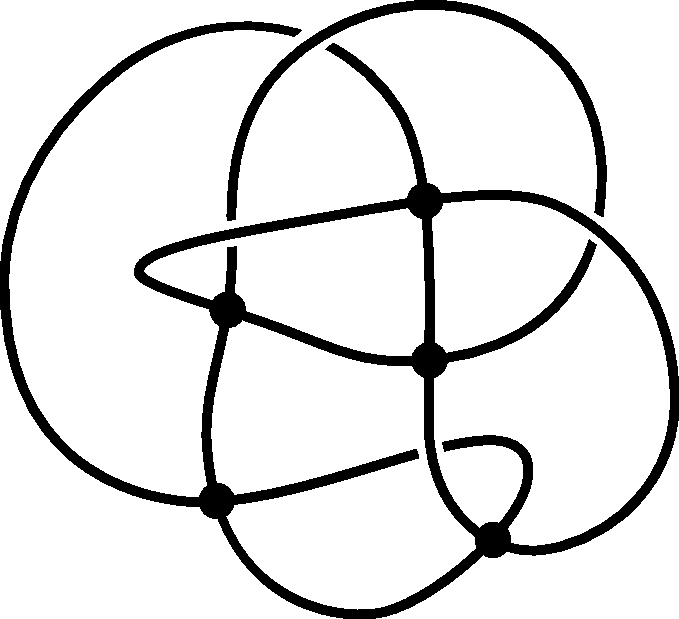
\includegraphics[width=0.14\textwidth, valign=c]{graphics/knot_9_33_singular.pdf}
		\quad \overset{\sigma}{\longmapsto} \quad
		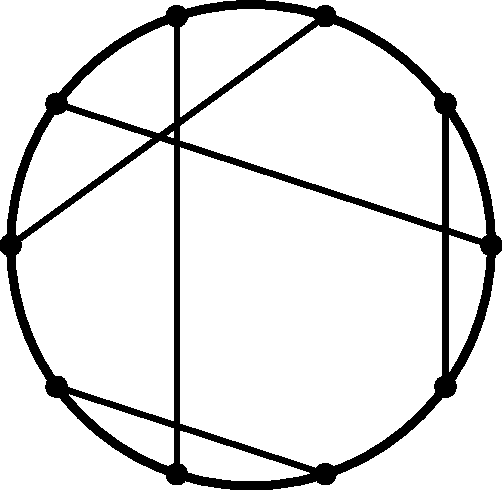
\includegraphics[width=0.13\textwidth, valign=c]{graphics/chord_diagram_of_knot_9_33_singular.pdf}
	\]
\end{example}

Given a functional

% TODO: Justify or motivate the quotient in the definition of the constants of integration. This leads to chord diagrams. Chord diagrams are exactly singular knots up to crossing change. Actuality tables and the full integration procedure. The Hutchings and Dror stuff about the secondart obstructions vanishing, and the fundamental theorem of Vassiliev invariants.
% TODO: Reformulation of the Weierstrauss conjecture as the fact that no knot invariant extends to contradict the relations. Perhaps the chord diagram ncatlab statements about cohomology.


\section{Third subsection}
